\section{Analisi del taglio e della flessione}	
	Come studiato in precedenza, la presenza dell'azione di taglio $\Tx,\Ty$ è sempre associata ad una variazione di momento flettente $\My,\Mx$ per via delle relazioni di equivalenza statica $T_y = \frac{d\Mx}{dz}$ e $T_x = - \frac{d\My}{dz}$. Per come visto a pagina \pageref{eq:sv:equivstatica} alle azioni di taglio sono associate le sole componenti di tensione $\txz,\tyz$ (che determinano delle distorsioni angolari $\gxz,\gyz$).
	
	A differenza di altre casistiche è necessario porre attenzione al fatto che le azioni $T_x,T_y$ e $M_z$ non sono necessariamente disaccoppiate, ossia per il teorema di Betti le azioni di taglio possono produrre un determinato lavoro per gli spostamenti dovuti alla torsione e viceversa. In linea generale queste \textbf{azioni} possono essere \textbf{trattate separatamente} solamente quanto sono energeticamente ortogonali, ossia presentano \textbf{lavoro mutuo nullo}. Questa condizione nella pratica si realizza solamente quando le azioni di taglio $T_x,T_y$ determinano una forza $\ov T = \Tx \vers i + \Ty \vers j$ che passa per il centro di taglio $C$ della sezione.
	
	Risolvere analiticamente in forma chiusa l'analisi al taglio risulta difficile e poco pratica per sezioni complesse, per questo tendenzialmente ci si limita a considerare sezioni a doppia/semplice simmetria, sezioni compatte e/o a spessore sottili, sezioni mono-connesse aperte o pluri-connesse chiuse.
	
	\paragraph{Analisi del taglio} Effettuare delle prove sperimentali di puro taglio è impossibile in quanto, come affermato in precedenza, allo stesso è sempre correlato una variazione di momento flettente.
	\figura{6}{1}{azioni-taglio}{diagramma dell'azione interna di taglio e momento flettente per una trave a sezione rettangolare incernierata a muro e caricata all'estremo opposto.}{azioni-taglio}
	
	Per analizzare dunque la risposta della trave si può dunque pensare di utilizzare, in maniera inversa, il principio di sovrapposizione degli effetti: nota la deformata reale del componente e potendo determinare la deformata a flessione della trave, per sottrazione è possibile ricavare la deformazione a puro taglio, come si può vedere in figura \ref{fig:taglio:schemadeformazione}.
	
	\begin{figure}[bht]
		\centering
		\begin{subfigure}{0.32\linewidth}
			\centering 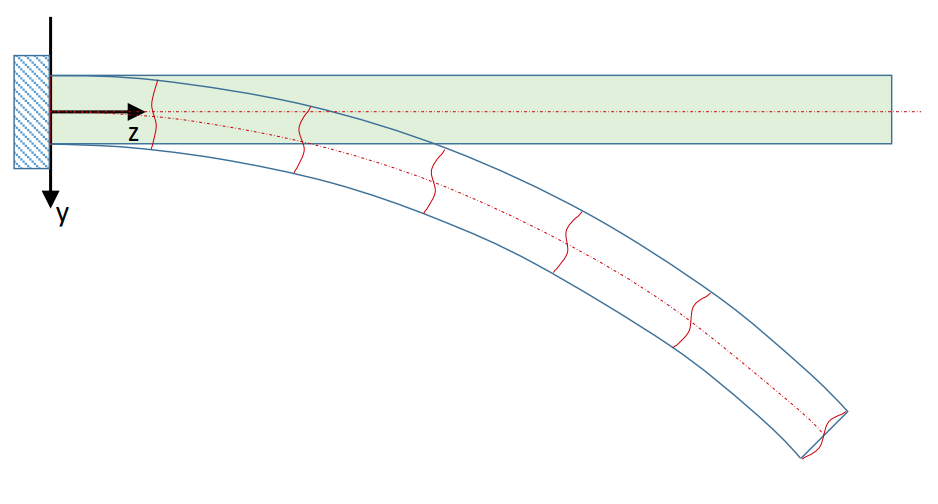
\includegraphics[width=0.9\linewidth]{taglio-a} \caption{}
		\end{subfigure}
		\begin{subfigure}{0.32\linewidth}
			\centering 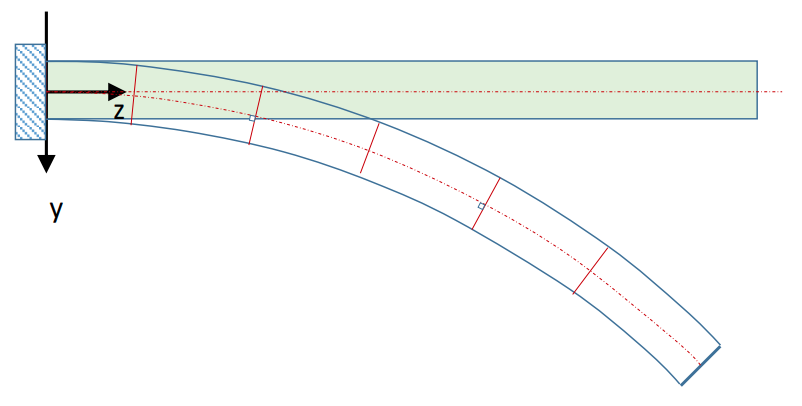
\includegraphics[width=0.9\linewidth]{taglio-b} \caption{}
		\end{subfigure}
		\begin{subfigure}{0.32\linewidth}
			\centering 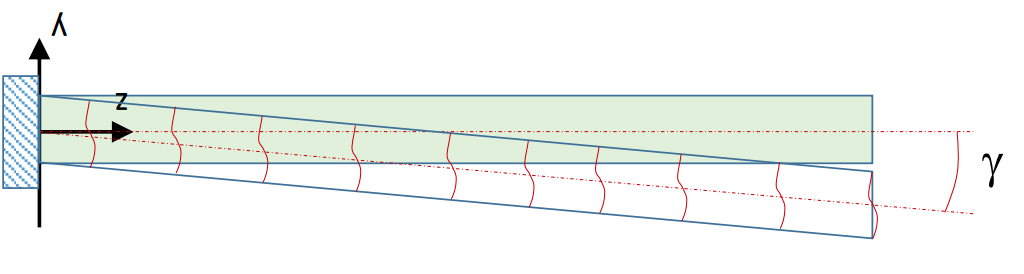
\includegraphics[width=0.9\linewidth]{taglio-c} \caption{}
		\end{subfigure}
		\caption{deformata totale di una trave di una trave sottoposta ad azione di taglio (a), deformata dovuta solamente al momento flettente (b) e conseguente deformata dovuta al solo taglio (c).}
		\label{fig:taglio:schemadeformazione}
	\end{figure}
	
	Si osserva che le sezioni non tendono a rimanere piane, ma sono soggette al fenomeno dell'ingobbamento già visto per la torsione, rappresentata in figura \ref{taglio-d}. In particolare l'azione di taglio non deforma l'asse (che dunque rimane rettilineo) e determina distorsioni angolari $\gxz,\gyz$ che sono nulle sul mantello, mentre risultano essere massime in corrispondenza del centro della sezione stessa.
	
	\figura{6}{1}{taglio-d}{effetto di distorsione della sezione dovuta all'azione di taglio}{taglio-d}
	
	La distorsione angolare è dovuta al fatto che è impedito lo scorrimento relativo tra le fibre longitudinali che compongono la trave, e dunque nascono delle azioni interne (con conseguenti deformazioni) che controbilanciano lo scorrimento. A tal proposito è dunque necessario, per il principio di reciprocità, determinare l'azione normale presente nella trave, che nel caso in questione vale
	\[ \szz = \frac{\Mx(z)}{\Ixx}y = -\frac{\Ty\big(L-z\big)}{\Ixx}y \]
	La presenza dell'azione $\szz$ rende il campo non solenoidale, ossia le linee di flusso della tensione $\ov \tau$ sono aperte.
	
	Per analizzare la distribuzione delle tensioni si farà prima riferimento alla cosiddetta \textbf{tensione retta}, ossia una tensione appartenente ad un asse principale di inerzia (una delle componenti $T_x,T_y$ deve dunque essere nulla), per poi combinare i risultati nella \textbf{tensione deviata}. 
	
	\subsection{Analisi del taglio retto con l'approccio di Jourawsky}
		Per studiare la risposta a taglio di una trave si utilizza l'\textbf{approccio approssimato di Jourawsky} il quale applica un'ipotesi semplificativa sull'andamento delle tensioni partendo da delle considerazioni di equilibrio di un volume elementare.
		
		Per rendere più facile l'analisi si parte a considerare il taglio retto applicato su una sezione a doppio asse di simmetria (che permette dunque di semplificare di fatto i calcoli) come mostrato in figura \ref{taglio-retto-a}.
		
		\figura{3}{2}{taglio-retto-a}{sezione a doppio asse di simmetria sottoposta a taglio retto $T_y$.}{taglio-retto-a}
		
		Le incognite del problema sono di fatto el componenti $\txz$ e $\tyz$ dello stato di tensione della trave; per poter determinare tali valori è necessario considerare le relazioni di equivalenza statica che, per come già visto in precedenza, permettono di affermare che
		\[ T_y = - \frac{d\Mx}{dz} \qquad \textrm e \qquad  \szz = -\frac{\Ty\big(L-z\big)}{\Ixx}y \quad \Rightarrow \quad \pd \szz z = \frac \Ty\Ixx y\]
		Con queste relazioni note è possibile riscrivere l'equilibrio indefinito (già visto a pagina \pageref{sec:sv:equilibrioindefinito}) del campo della trave tramite l'equazione differenziale
		\begin{equation} \label{eq:taglio:temp1}
			\pd \txz x + \pd \tyz y = -\pd \szz z = - \frac \Ty \Ixx y
		\end{equation}
		\begin{nota}
			Questo dimostra la non solenoidalità del campo delle tensioni $\ov \tau$ in quanto si dimostra che $\textrm{div}(\ov \tau) =- \frac \Ty \Ixx y \neq 0$.
		\end{nota}
		
		A questo punto per continuare l'analisi tramite il metodo di Jourawsky si sceglie una corda (la cui lunghezza vale $b(y)$ ) qualsiasi perpendicolare all'asse $y$ dove giace l'azione di taglio, ossia determinata (in funzione della coordinata $y$) dai punti
		\[ P_1 = \left(\frac{b(y)}{2}, y\right) \qquad P_2 = \left(-\frac{b(y)}{2}, y\right) \]
		L'andamento delle tensioni $\txz \parallel \ov P_1\ov P_2$ e $\tyz \perp \ov P_1\ov P_2$ non risulta essere noto a priori, tuttavia è possibile supporre che il loro valore sia pressoché costante, e dunque si determina le media integrale di tali grandezze:
		\[ \tau_{yz,m}= \frac 1 {b(y)} \int_{-b/2}^{b/2} \tyz \, dx \qquad \tau_{xz,m}= \frac 1 {b(y)} \int_{-b/2}^{b/2} \txz \, dx = 0  \]
		\figura{3.5}{2}{taglio-retto-b}{tensioni $\txz,\tyz$ e coordinate generalizzate usate per l'analisi del taglio retto.}{taglio-retto-b}
		
		In particolare essendo la sezione simmetrica e la tensione verso solo l'asse $y$, per l'equivalenza statica con $T_x$ è necessario imporre la media integrale del campo scalare $\txz$ come nulla.
		
		\begin{concetto}
			L'\textbf{ipotesi semplificativa di Jourawsky} si basa sul fatto di considerare il campo $\tyz$ costante lungo tutta la corda della sezione perpendicolare all'asse $y$ e pari al valor medio $\tyz = \tau_{yz,m}$; al contrario il valor medio $\tau_{xz,m}$ deve essere nullo.
		\end{concetto}
		
		A questo punto è necessario determinare un \textit{metodo} per calcolare il valor medio della tensione lungo la corda della sezione. A tal fine si considera l'\textbf{area sottesa alla corda} $A^*$ e il concio elementare che essa genera, come in figura \ref{taglio-retto-c}. Partendo da tale diagramma è possibile osservare come, per reciprocità, la componente di tensione $\tyz$ presenta anche un'azione applicata parallelamente all'asse $z$ (direzione dell'azione $\szz$).
		
		\figura{5}{1.3}{taglio-retto-c}{volume elementare estratto dall'area sottesa $A^*$ alla corda; l'ultima immagine rappresenta anche i conci elementari adiacenti a quello considerato per effettuare il bilancio delle azioni interne.}{taglio-retto-c}
		
		Si può dunque osservare che in corrispondenza della faccia $AB$ agisce una forza $\szz$ (dovuta alle azioni di superficie sul concio elementare), mentre su $CD$ si ha un'azione pari a $\szz + \pd \szz z dz$; in particolare la risultante netta $dN$ dovuta all'azione interna normale può essere calcolata noto che la variazione $\pd \szz z$ coincide, per come visto nell'equazione \ref{eq:taglio:temp1}, con la funzione $-\frac \Ty\Ixx y$ e dunque
		\[ dN = \int_{A^*(y)} \pd \szz z \, dz\, dA = \int_{A^*(y)} \pd Ty \Ixx y \, dz \, dA \]
		
		\begin{concetto}
			Questa forza deve dunque essere contro-bilanciata dall'azione reciproca di $\tyz$ che, in questo caso, risulta valere $dF = \tau_{yz,m} b(y)\, dz$: eguagliando dunque i termini $dN = dF$ è possibile esplicitare il valor medio della componente $\tyz$, che prende il nome di \textbf{tensione di Jourawsky}, dell'area sottesa $A^*$ tramite l'espressione
			\begin{equation} \label{eq:taglio:retto}
				\tau_{yz,m} = \frac{\Ty  }{\Ixx \, b(y)}\int_{A^*} y\, dA  = \frac{\Ty  }{\Ixx} \frac {S_x^*(y)}{ b(y)}
			\end{equation}
		\end{concetto}
		Si può dunque osservare che l'integrale $\int_{A^*}y\,dA = S_x^*$ rappresenta il momento statico dell'area $A^*$ valutato rispetto all'asse $x$; in questa espressione va notato come il rapporto $T_y/\Ixx$ sia una proprietà fissa della trave, mentre $S_x^*/b$ è una funzione dipendente dalla posizione $y$ rispetto alla quale si sceglie di posizionare la corda (infatti variando $y$ varia sia l'area che determina il momento statico, sia in generale la lunghezza della corda stessa).
		\figura{3.5}{2}{taglio-retto-d}{azioni $dN$ dovute alle azioni interne e $dF$ dovute alle azioni di taglio.}{taglio-retto-d}
		
		Avendo considerato la sezione della trave come doppiamente simmetrica, allora è possibile verificare la condizione di componente $\tyz$ nulla al contorno del mantello: tale considerazione è basata sul calcolo del momento statico rispetto alle coordinate massime e minime di $y$, e dunque
		\[ \textrm{per } y = \begin{cases}
			y_{max} \qquad \rightarrow \quad A^* = 0 \qquad \Rightarrow \quad S^* = 0 \qquad \Rightarrow \quad \tau_{yz,m} = 0 \\
			y_{min} \qquad \rightarrow \quad A^* = A \qquad \Rightarrow \quad S^* = 0 \qquad \Rightarrow \quad \tau_{yz,m} = 0 \\
		\end{cases}\]
		
		\paragraph{Componente normale all'azione di taglio} Fino ad ora è stato mostrato il processo che permette di calcolare la tensione $\tyz$, assunta come costante e pari al valore medio, dovuta all'azione di taglio dipendente dalla posizione della corda che si vuole scegliere (il risultato è quello esposto nell'equazione \ref{eq:taglio:retto}). Tuttavia quello che resta da definire è il valore della componente $\txz$ che di fatto dovrà garantire la condizione di tangenza del campo $\ov \tau$ al mantello.
		
		L'espressione di tale componente può essere determinata, partendo dalla tensione di Jourawsky, derivando lungo l'asse $x$ l'espressione \ref{eq:taglio:temp1}: osservando che la componente $\txz$ è indipendente dalla posizione $z$ che si sta considerando, allora per integrazione si determina che
		\[ \textrm{eq \ref{eq:taglio:temp1}}\xrightarrow{\pd {}x } \pd{^2\txz}{x^2} = 0 \qquad \xrightarrow{\textrm{ integrazione }} \quad \txz = A(y) x + B(y)  \]
		A questo punto per determinare i coefficienti $A,B$ dipendenti dalla posizione $y$ della corda è necessario imporre le condizioni al contorno; noto il versore $\vers n_\Gamma = (\alpha_x,\alpha_y)$ normale al mantello imponendo il prodotto scalare $\ov \tau \cdot \vers n_\Gamma$ nullo (condizione di perpendicolarità) è possibile ricavare che
		\[ \txz \alpha_x + \tyz \alpha_y = 0\qquad \Rightarrow \quad \txz = -\frac{2x}{b} \frac{\alpha_y}{\alpha_x} \tyz \]
		
		\paragraph{Generalizzazione} La teoria formulata da Jourawsky si basa di fatto sulla formulazione dell'equilibrio di un volume elementare che in generale può essere determinato da una corda non necessariamente ortogonale all'azione di taglio retto, come si può osservare in figura \ref{taglio-retto-gen}. L'analisi di questo tipo di problema è analoga a quanto visto fino ad ora, tuttavia è necessario considerare il sistema di riferimento ruotato di assi $q,\lambda$ e dunque calcolare la componente
		\[\tlz = \frac{\Ty S_x^*(y)}{\Ixx b(y)}\]
		
		\figura{5}{1.2}{taglio-retto-gen}{analisi degli stati di tensione per corde non perpendicolari all'azione $T_y$.}{taglio-retto-gen}
		
		E' inoltre possibile asserire delle considerazioni sul \textbf{verso} della tensione $\tyz$: scelta infatti l'area $A^*$ se si calcola $\tlz > 0$, allora la tensione è \textbf{entrante nell'area} $A^*$ che si sta considerando, mentre al contrario se $\tyz < 0$ il verso è opposto e dunque uscente dall'area.
		
	\subsection{Analisi del taglio deviato}
		In generale una trave non è sottoposta ad un'azione di taglio puramente retto, ma è soggetta ad un \textbf{taglio deviato} (cui è associato un momento deviato) in quanto è possibile considerare l'azione tagliante come
		\[\ov T = \Tx\vers i + \Ty \vers j\]
		In particolare per quanto riguarda la flessione deviata ne è nota la formulazione esplicita del campo scalare $\szz$ (pag. \pageref{sec:fless:deviata}) e dunque è possibile ricavarne la derivata rispetto alla coordinata assiale:
		\[ \pd \szz z = \frac \Ty \Ixx y + \Tx \Iyy x \]
		Sfruttando un ragionamento analogo al calcolo del taglio retto è possibile determinare la componente $\tyz$ della tensione $\ov \tau$ scegliendo una corda perpendicolare all'asse $y$ e valutando gli integrali rispetto all'area sottesa a tale linea, e dunque
		\begin{equation} \label{eq:taglio:deviato}
			\tyz = \frac 1 {b(y)} \left(\frac \Ty \Ixx \int_{A^*} y\, dA + \frac \Tx \Iyy \int_{A^*} x\, dA\right) = \frac 1  {b(y)} \left(\frac{\Ty S_x^*(y)}{\Ixx} + \frac{\Tx S_y^*(y)}{\Iyy} \right)
		\end{equation}
		\begin{nota}
			Per travi a sezione simmetriche è possibile osservare che i momenti statici sono nulli rispetto agli assi di simmetria; questo significa, per esempio, che la componente $\tyz$ di una trave a sezione doppiamente simmetrica lungo gli assi $x,y$ dipende solamente dalla componente $T_y$ (in quanto a $T_x$ è associato il momento $S_y^*$ che è sempre nullo).
		\end{nota}
		
	\subsection{Sezioni piene a geometria semplice}
	\subsubsection{Sezione rettangolare}
		Considerando una sezione rettangolare di dimensione orizzontale $b$ (lungo l'asse $x$) e dimensione verticale $h$, essendo la sezione doppiamente simmetrica allora il centro di taglio coincide con il baricentro e le azioni taglianti sono disaccoppiate.
		
		\figura{4}{2}{taglio-rettangolo-a}{sezione rettangolare di una trave e coordinate principali di riferimento.}{taglio-rettangolo-a}
		
		Considerando di applicare solamente un'azione di taglio $\Ty$, per calcolare lo stato di tensione $\tyz$ ad essa associato è sufficiente calcolare i parametri geometrici della sezione e le variabili in $y$ in maniera esplicita. In particolare il momento di inerzia rispetto all'asse orizzontale vale $\Ixx = \frac 1 {12}bh^3$; la lunghezza della corda parallela all'asse $x$ sarà sempre costante e pari a $b(y) = b$. A questo punto è necessario calcolare il momento statico $S^*_x(y)$ determinato come il prodotto della posizione del baricentro dell'area $A^*$ per il valore dell'area stessa:
		\[y_c = \frac 12\left( \frac h 2 + y\right) \quad A^* = b \left(\frac h 2 - y \right) \qquad \Rightarrow \quad S_x^* = A^* y_c = \frac{bh^2}{8} \left[ 1 - \left(\frac{2y}{h}\right)^2 \right]\]
		Avendo determinato tutti gli elementi costitutivi dell'equazione \ref{eq:taglio:retto} (pag. \pageref{eq:taglio:retto}) è sufficiente determinare l'espressione esplicita dello stato di tensione che vale dunque
		\begin{equation}
			\tyz = \frac{\Ty S_x^*}{\Ixx b} = \frac 3 2 \frac \Ty{bh}  \left[ 1 - \left(\frac{2y}{h}\right)^2 \right]
		\end{equation}
		
		Da questa relazione si evince che il valore di massimo della componente di tensione $\tyz$ è associata al valore massimo del momento statico che è associato alla quota $y=0$ e dunque
		\[\tau_{yz,max} = \tyz(0) = \frac 3 2 \frac \Ty A\] 
		\begin{concetto}
			Per le sezioni più comuni si tende a definire il \textbf{fattore di taglio} $\eta_t$ come il rapporto tra la tensione massima nella sezione calcolata tra Jourawsky e la tensione che si dovrebbe avere nominalmente $\tau_{yz,nom} = T_y/A$; nel caso particolare di sezione rettangolare si dimostra che
			\begin{equation} \label{eq:taglio:fattore}
				\tau_{yz,max} = \frac 3 2 \frac \Ty A \quad \tau_{yz,nom} = \frac \Ty A \qquad \Rightarrow \quad \eta_t = \frac{\tau_{yz,max}}{\tau_{yz,nom}} = \frac 3 2
			\end{equation}
		\end{concetto}
		
		Dall'analisi delle condizioni al contorno (e anche a livello intuitivo) si osserva che la componente $\txz$ (associata al solo taglio $T_y$) è sempre nulla lungo tutta la corda considerata.
		
		Il valore della componente $\tyz$ (al variare di $y$) assume una forma parabolica (con valore massimo per $y=0$ e valore nullo agli estremi del rettangolo), come si può vedere in figura \ref{taglio-rettangolo-b}; inoltre nelle operazione di verifica/resistenza è necessario considerare anche l'effetto del campo $\szz$ che può essere calcolata in maniera analitica noto che
		\[ \szz = \frac \Mx \Ixx y = -\frac{\Ty\big( L-z \big)}{\Ixx} y \qquad \Rightarrow \quad \sigma_{zz,max}= - \frac{12\Ty\big( L-z \big) }{bh^2}\]
		
		Si osserva dunque che in generale, essendo $L,z \gg b,h$, nelle operazioni di verifica/dimensionamento la condizione più stringente è determinata dalla tensione normale $\szz$ associata alla flessione (e dunque in generale il taglio si trascura).
		
		\figura{7}{1}{taglio-rettangolo-b}{profili delle componenti $\tyz$ e $\szz$ della tensione di una trave a sezione rettangolare soggetta a taglio retto $\Ty$.}{taglio-rettangolo-b}
		
		L'ipotesi di Jourawsky si basa sull'assumere la distribuzione della tensione $\tyz$ come costante lungo tutta la corda, tuttavia nella realtà è possibile osservare degli scostamenti, anche significativi, nella distribuzione delle tensioni, in particolare nel valutare il valore massimo della componente di tensione per effettuare verifiche e dimensionamenti. In particolare per rapporti $b/h$ inferiori al valore $1/2$ l'errore che si commette a valutare il picco di tensione è pari al $3\%$, e dunque si può trascurare. Alzando il rapporto $b/h = 2$ l'errore tra valore reale e nominale aumenta al $40\%$ e l'errore è maggiore del $100\%$ per $b/h>4$.
		
	\subsubsection{Sezione circolare}
		Si consideri ora una trave a sezione circolare mostrata in figura \ref{taglio-circolare-a} sottoposta al solo taglio $T_y$. Per semplificare l'analisi si preferisce ricondurre tutte le grandezze in funzione dell'angolo $\phi$ al centro mostrato.
		\figura{3.2}{2}{taglio-circolare-a}{schema di riferimento per l'analisi a taglio di una trave a sezione circolare.}{taglio-circolare-a}
		
		Così facendo è possibile esprimere la quota $y$ della corda in funzione del raggio tramite la relazione $y = R\cos\phi$; dall'analisi è anche possibile calcolare la lunghezza della corda $b(\phi) = 2R \sin\phi$ e il momento statico dell'area sottesa $S_x^* = \frac 2 3 \big(R\sin\phi\big)^3$. Essendo noto il momento d'inerzia $I_{xx} = \frac pi 4 R^4$ allora si può calcolare la componente di tensione $\tyz$ che risulta valere
		\begin{align*}
			\tyz &  = \frac {\Ty S_x^*}{b\,\Ixx} = \frac 4 3 \Ty \frac{\sin^2\phi}{\pi R^2} = \frac 4{3\pi} \frac \Ty {R^2} \left(1-\cos^2\phi\right) \\
			&  = \frac 4{3\pi} \frac \Ty {R^2} \left(1-\frac{y^2}{R^2}\right)
		\end{align*}
		Anche in questo caso l'andamento del modulo della tensione $\tyz$ presenta un andamento parabolico con valore massimo alla quota $y = R$ e valore nullo per $y = \pm R$. Si evince dunque che il fattore di taglio (eq. \ref{eq:taglio:fattore}) per la sezione circolare vale
		\[ \eta_t = \frac{\tau_{yz,max}}{\tau_{yz,nom}} = \frac 4 3  \]
		
		\vspace{3mm}
		A questo punto è necessario analizzare le componenti $\txz$ che rendono il campo $\ov\tau$ tangente al mantello in ogni punto della sezione; noto che il versore $\vers n_\Gamma = (\alpha_x,\alpha_y)$ dipende dall'angolo $\phi$ e che vale $\alpha_y/\alpha_x= 1/\tan\phi$, imponendo le condizioni al contorno si osserva che
		\begin{align*}
			\txz & = -\frac {2x}b\tyz \frac{\alpha_x}{\alpha_y} = - \frac{2x}{b} \frac 4 3 \frac \Ty A \sin^2\phi \frac 1 {\tan\phi} \\
			\xrightarrow{x = b/2 = R\sin\phi} & = -\frac 4 3 \frac{\Ty}{\pi R^2}\sin\phi\cos\phi	
		\end{align*}
		
		Con i risultati ottenuti è dunque possibile esprimere il valore del modulo $\tau$ dello stato di tensione in funzione dell'angolo $\phi$, osservando che si ha valore massimo in corrispondenza di $\phi = \frac \pi 2$:
		\[\tau = \sqrt{\txz^2+\tyz^2} = \frac 4{3} \frac{\Ty}{\pi R^2} \sin\phi \qquad \xrightarrow{\phi = \pi/2} \quad \tau_{max} = \frac 4 3 \frac \Ty A \]
		Anche in questo caso, come per la sezione rettangolare piena, nel calcolo a resistenza/verifica il valore del campo $\ov \tau$ a taglio risulta irrisoria rispetto al campo $\szz$ dovuto alla flessione.
		
	\subsection{Sezioni aperte a parete sottile}
		L'analisi a taglio di una trave con sezione a parete sottile aperta si basa, come si può osservare in figura \ref{taglio-sottile}, sulla corda $b(\lambda)$ (con $\lambda$ coordinata curvilinea della sezione) sviluppata perpendicolarmente alla linea media $\Gamma$ della sezione.
		
		Per evitare effetti torsionali si ipotizza di conoscere il centro di taglio $C$ e si richiede che il taglio $\ov T = \Tx \vers i + \Ty \vers j$ passi per tale punto.
		
		\figura{4}{2}{taglio-sottile}{schema di riferimento per l'analisi a taglio di una trave di sezione aperta a parete sottile.}{taglio-sottile}
		
		Per l'analisi dello stato di tensione è più pratico utilizzare il sistema di riferimento locale, dipendente dalla coordinata $\lambda$, che determina le componenti $\tlz$ perpendicolare alla corda (e dunque approssimativamente parallela al mantello) e la componente $\tau_{qz}$ giacente sulla corda, il cui effetto si trascura in quanto deve essere nulla ai bordi per le condizioni al contorno (ed essendo la parete sottile si ipotizza che il valore sia pressoché uniforme).
		
		La componente $\tlz$ può essere definita a partire dall'espressione $\ref{eq:taglio:deviato}$ (pag. \pageref{eq:taglio:deviato}) che permette di definire il \textbf{flusso di taglio} $\plz$:
		\[\tlz = \frac 1{b(\lambda)} \left( \frac{\Ty S_x^*(\lambda)}{\Ixx} + \frac{\Tx S_y^*(\lambda)}{\Iyy} \right) \qquad \Rightarrow \quad \plz = \tlz b(\lambda) = \frac{\Ty S_x^*(\lambda)}{\Ixx} + \frac{\Tx S_y^*(\lambda)}{\Iyy} \]
		A differenza della torsione, è possibile osservare che il flusso di taglio $\plz$ non è costante lungo la sezione, ma dipende strettamente dalla coordinata curvilinea $\lambda$.\\
		Tale effetto si può dimostrare considerando, come nella teoria di Bredt, l'equilibrio del tratto elementare osservando che all'equilibrio si ha l'effetto di una tensione normale $dN$ dovuta a $\szz$ che produce una risultante netta.
		
		La direzione del flusso può essere determinata a livello intuitivo come quello di un fluido che dovrebbe scorrere in un contenitore coincidente con la sezione e la cui direzione del fluido dipende da $\ov T$.
		
	\subsubsection{Sezione a doppia T}
		Si consideri il caso della sezione a doppia T mostrata in figura \ref{doppia-T}: in questa situazione la tensione $\tlz$ dipendente dalla coordinata curvilinea della sezione è associata alla sola componente $\txz$ lungo le \textbf{ali}, mentre nell'anima vale $\tlz = \tyz$.
		\figura{4}{2}{doppia-T}{esempio di sezione a doppia T con dimensioni "principali".}{doppia-T}
		In figura \ref{taglio-T-a} è possibile osservare come, tramite l'analogia del fluido, il flusso delle tensioni si distribuisce per le due azioni di carico retto lungo le direzioni principali.
		
		\figura{7}{1}{taglio-T-a}{flussi di tensione per taglio retto $\Ty$ (a sinistra) e $\Tx$ (a destra).}{taglio-T-a}
		
		Si parta a considerare l'azione $\Ty$ cui è associato il momento flettente $\Mx$ (distribuzione mostrata in figura \ref{taglio-T-b}). Considerando la metà sinistra dell'ala superiore, partendo dal punto $A_1$, è possibile osservare che il momento statico $S_x^*$ dipendente dalla coordinata $\lambda_1$ vale $\lambda_1 b_1 \frac H 2$. A questo punto si determina $\tlz = \txz$ che risulta valere
		\[ \txz = \frac {\Ty S_x^*}{b\Ixx} = \frac{\Ty \lambda_1 b_1 H/2}{I_{xx,1}b_1} = \frac{\Ty H}{2 I_{xx,1}} \lambda_1 \]
		In maniera speculare è possibile determinare lo stato $\txz$ per la parte destra dell'ala superiore. Il valore massimo dello stato di tensione si ha in corrispondenza della coordinata $\lambda_1 = \lambda_2 = B/2$ con un valore di 
		\[ \tau_{xz,1,max} = \frac{\Ty BH}{4 I_{xx,1}b_1} \]
		\figura{5}{1.5}{taglio-T-b}{schema di riferimento per la determinazione dello stato di tensione dovuto a $T_y$ e distribuzione associata al momento $M_z$.}{taglio-T-b}
		\figura{6}{2}{taglio-T-c}{due metodi di rappresentazione della tensione sull'ala del profilo a doppia T: a sinistra si rappresenta a diagramma il modulo della tensione e si correla il verso delle tensioni (tramite le frecce), mentre nel secondo metodo il diagramma di azione interna rappresenta modulo e verso dell'azione.}{taglio-T-c}
		
		Considerando invece la parte dell'anima, il momento statico $S_x^*(y)$ può essere valutato per via integrale e dunque determinare lo stato di tensione
		\[ S_x^*(y) = b_1 B\frac H2 + \int_y^{H/2}b_2y'\, dy' = b_1 B \frac H 2 + b_2 \left(\frac{H^2}{8} - \frac{y^2}{2}\right)  \]
		Si osserva dunque che il profilo della tensione $\tyz$ assume forma parabolica e in particolare il valore agli estremi dell'anima coincide con la somma dei flussi di tensione entranti dalle ali. Considerando infatti che i flussi delle tensioni sulle ali valgono $\Phi_{xz,1} = \Phi_{xz,2} = \frac \Ty\Ixx \frac{BH}{4}b_1$ e $\Phi_{yz,3} = \frac \Ty {2\Ixx} \frac{BH} 4 b_1$, allora si osserva che
		\[ \Phi_{xz,1} + \Phi_{xz,2} = \Phi_{yz,3} \]
		\figura{5}{1.5}{taglio-T-d}{distribuzione del modulo della tensione $\tlz$ lungo le varie parti che compongono la sezione a doppia T.}{taglio-T-d}
		
		Come è possibile osservare in figura \ref{taglio-T-d}, il punto critico in cui si ha la concentrazione delle azioni di tensione sono le giunture tra anima e ali della sezione: in questa zona si ha di fatto una perturbazione dello stato di tensione il cui modulo effettivo, in valore assoluto, può essere valutato tramite il \textbf{coefficiente di Treffetz} $K$ (dipendente dallo spessore $b$ dell'anima e dal raggio di raccordo $\rho$ tra anima e ali):
		\[K = \frac{\tau_{\lambda z,reale}}{\tlz} = \max\left\{  1.74 \sqrt{\frac b\rho},1 \right\}  \]
		
		\vspace{3mm}
		Considerando ora la sezione come sottoposta solamente a taglio $\Tx$, facendo riferimento allo schema riportato in figura \ref{taglio-T-e}, è possibile determinare il momento statico $S_y^*$ utile a determinare il campo $\tlz = \txz$ sulle ali della sezione:
		\[ S_y^*(x) = \int_{A^*} x \, dA = b_1\left( \frac B 2 -x\right) \left(\frac B 2 + x\right) \qquad \Rightarrow \quad \tlz = \frac{\Tx}{\Iyy b_1}\left[\frac{b_1}{2} \left(\frac{B^2}{4}-x^2\right) \right] \]
		Si osserva così che il profilo della tensione $\txz$ sulle ali assume forma parabolica con valore nullo agli estremi e valore massimo nel centro della sezione pari a $\frac \Tx \Iyy \frac {B^2}8$. Analizzando l'anima invece, essendo tale sezione simmetrica rispetto all'asse $y$, si evince che il momento $S_x^*$ è sempre nullo e dunque $\tlz = 0$ in ogni punto.
		\figura{5}{1.5}{taglio-T-e}{schema di riferimento per la determinazione dello stato di tensione dovuto all'azione di taglio $T_x$.}{taglio-T-e}
	
	\subsubsection{Sezioni aperte a parete sottile non simmetriche}
		Nel caso più generico di una sezione (non doppiamente simmetrica) il cui carico non passa per il centro di taglio, allora è possibile osservare che si ha la formazione di uno stato di tensione, che oltre a quello di taglio studiato da Jourawsky,  è dovuto alla torsione.
		
		Per capire questo tipo di effetto si consideri la \textbf{sezione a C}, a semplice simmetria, il cui schema è mostrato in figura \ref{taglio-C-a}.
		
		\figura{6.5}{1}{taglio-C-a}{schema di riferimento (a sinistra) e distribuzione delle tensioni (a destra) di una sezione a C.}{taglio-C-a}	
		
		Analizzando lo stato di tensione di Jourawsky, tramite l'equazione \ref{eq:taglio:deviato} (pag. \pageref{eq:taglio:deviato}), è possibile ricavare in maniera esplicita le tensioni sull'anima (solo componente $\tyz$) e sulle ali ($\txz$) nel caso di sola azione $\Ty$ secondo le equazioni
		\[ \textrm{anima: } \tyz = \frac \Ty \Ixx \left[ \frac{HBb_1}{2b_1} + \left(\frac {H^2}4 - y^2\right) \right] \qquad \textrm{ali: } \txz =\frac \Ty\Ixx \frac H 2 \lambda_1 \]
		Si giustifica così il profilo lineare delle tensioni sulle ali e l'andamento parabolico sull'anima delle tensioni mostrato in figura \ref{taglio-C-a}.
		\begin{nota}
			In questo caso la simmetria della sezione è rispetto all'asse $x$, e dunque non ha senso studiare il taglio associato $\Tx$ in quanto, passando per il centro di taglio, non genererebbe alcuna azione torcente.
		\end{nota}
		
		Integrando lo stato di tensione sull'asse è possibile osservare che lo stesso determina delle azioni risultanti $F_1,F_2$ (la cui posizione e verso di applicazione è mostrato in figura \ref{taglio-C-b}) di valori
		\[ F_1 = \frac \Ty \Ixx \frac{HB^2}{4}b_1 \qquad F_2 = \Ty \]
		
		\figura{3}{2}{taglio-C-b}{forze determinate dallo stato di tensione $\tlz$ dovuto al taglio $\Ty$.}{taglio-C-b}	
		
		Si osserva così che la risultante di tali forze coincide effettivamente all'azione di taglio $\Ty$ della sezione, tuttavia rispetto al baricentro le tensioni sulle ali determinano una coppia di forze pari a
		\[ \Mz = 2 F_1 \frac H 2 = \frac \Ty \Ixx \frac{H^2B^2}{4}b_1 \]
		Tramite delle relazioni di equivalenza statica è possibile calcolare l'\textbf{eccentricità} $e$ dell'azione $\Ty$ che permette di modellare, oltre allo stato tensionale di taglio, anche gli effetti di torsione, definendo di fatto la posizione \textbf{centro di taglio} $C$:
		\[ e = \frac \Mz \Ty = \frac{H^2B^2b_1}{4\Ixx} \]
		\figura{7.5}{1}{taglio-C-c}{equivalenza statica che permette di determinare il centro di taglio.}{taglio-C-c}	
		
		A questo punto per concludere l'analisi dello stato di tensione è possibile sfruttare il principio di sovrapposizione degli effetti: considerando infatti un tratto della sezione lo stato di tensione $\ov \tau$ sarà determinato dal contributo costante dovuto alla tensione di Jourawsky, mentre sarà anche presente un contributo \textit{triangolare} dovuto al momento torcente $\Mz$ (determinato dal fatto che $\Ty$ non fosse applicata nel centro di taglio).
		
		\begin{osservazione}
			Sezioni formate dall'unione di più lati rettilinei in un solo punto presentano centro di taglio coincidente con l'intersezione delle sezioni stesse.
		\end{osservazione}
		
	\subsection{Sezioni chiuse a parete sottile}
		Lo studio delle sezioni chiuse a parete sottile è più complesso in quanto le sole ipotesi (e relativo metodo) di Jourawsky non sono sufficienti a studiare completamente il problema. In generale per studiare una sezione biconnessa ci si riconduce ad una struttura monoconnessa 	\textit{tagliando} in un punto la sezione imponendo successivamente una compatibilità cinematica per garantire la continuità della sezione stessa.
		
		Nel caso particolare di \textbf{sezioni simmetriche} l'analisi risulta notevolmente semplificata in quanto è possibile ipotizzare che lo stato di tensione $\tlz$ si distribuisce in maniera speculare nella sezione rispetto all'asse di simmetria, e in particolare i flussi $\plz$ devono rimanere uguali lungo le due sotto-sezioni monoconnesse.
		
		\figura{3.5}{2}{taglio-chiusa}{schema di riferimento per l'analisi al taglio di una sezione chiusa a parete sottile.}{taglio-chiusa}
		
		Facendo particolare riferimento allo schema in figura \ref{taglio-chiusa} che assume valenza generale, è possibile affermare che i flussi $\Phi_{\lambda z,1}$ e $\Phi_{\lambda z,2}$ debbano essere uguale, e dunque
		\begin{equation}
			\Phi_{\lambda z,1} = \Phi_{\lambda z,2} = \frac{\Ty S_x^*}{2\Ixx} \qquad \Rightarrow \quad \tau_{\lambda z,1} = \tau_{\lambda z,2} = \frac{\Ty S_x^*}{2\Ixx b}
		\end{equation}
		\begin{nota}
			In questo caso è mostrata la risposta della sezione al solo taglio $\Ty$, ma lo stesso concetto può essere esteso al taglio $\Tx$ e dunque al taglio deviato.
		\end{nota}
	
	\subsection{Campo di deformazione}
		Come già iniziato a vedere in figura \ref{fig:taglio:schemadeformazione} (pag. \pageref{fig:taglio:schemadeformazione}) depurando dalla deformata complessiva il campo dovuto alla sola componente di flessione, è possibile osservare che la deformata del solo taglio non varia la conformazione dell'asse (che pertanto rimane rettilineo) ma ne cambia solamente l'\textit{inclinazione}.
		
		In particolare anche in questo caso è possibile fare riferimento ai \textbf{campi di spostamento}:
		\begin{itemize}
			\item \textbf{primario}, associato alla variazione di inclinazione dell'asse. Noto infatti l'angolo di inclinazione $\gamma$ dell'asse deformato si determina la componente del campo $v$ dovuta al taglio secondo la relazione
			\[ v = \gamma z\]
			Da ciò si evince che lo scostamento verticale massimo sarà in corrispondenza dell'estremità, ossia $v_{max} = v(L) = \gamma L$;
			\item \textbf{secondario}, dovuto all'effetto di ingobbamento, il cui effetto generalmente può essere trascurato in quanto il valor medio di scostamento $w$ dei punti della sezione è nullo
			\[ w_\textrm{medio}  = 0 \]
		\end{itemize}
		\figura{7}{1}{taglio-def}{deformata di una trave dovuta al solo taglio, ossia depurata dalla deformata a flessione.}{taglio-def}
		
		\begin{osservazione}
			In generale si osserva che i contributi dei campi $u,v$ a taglio possono essere trascurati per le travi in quanto per $L\gg H$ (con $H$ dimensione caratteristica della sezione) tali valori sono di molto inferiori rispetto ai campi dovuti alla flessione (derivante dal taglio stesso).
		\end{osservazione}
		
		\paragraph{Considerazioni energetiche} Considerando che l'unica azione applicata nella trave di esempio (figura \ref{taglio-def}) sia una componente $T_y$ applicata all'estremità, allora è possibile analizzare la deformata tramite il teorema di Clapeyron, ossia confrontando il lavoro delle forze esterne con l'energia elastica:
		\[ \underbrace{\frac 1 2 \Ty v(L) = \frac 1 2 \Ty \gamma L }_{L_{ext}} = \underbrace{\int_V \psi\, dV = \frac L {2G} \int_A \tau^2\, dA }_{U_e} \]
		\begin{concetto}
			Derivando quest'ultima relazione rispetto alla coordinata assiale è possibile così stabilire la variazione infinitesima dell'energia elastica lungo l'asse:
			\begin{equation} \label{eq:taglio:der-energia}
				\frac{dU_e}{dz} = \frac 1 2 \Ty \gamma = \frac 1 {2G}\int_A \tau\, dA
			\end{equation}
		\end{concetto}
	
		Tramite l'analisi di Jourawsky è stato possibile calcolare in maniera esplicita il valore della tensione $\tlz$ dipendente dal taglio $\Ty$ (eq. \ref{eq:taglio:retto}, pag. \pageref{eq:taglio:retto}), e dunque questo ci permette di definire in maniera esplicita la relazione tra angolo di deformazione $\gamma$ e taglio applicato $\Ty$. Considerando l'esempio della sezione rettangolare è possibile esprimere il campo della tensione come		
		\[ \tlz = \frac{\Ty  }{\Ixx} \frac {S_x^*(y)}{ b(y)} = \frac \Ty \Ixx R(x,y) \qquad \textrm{ con } R(x,y) = \frac 1 2 \left( \frac{H^2}{4} - y^2 \right) \]
		\begin{nota}
			In generale $R(x,y)$ rappresenta il rapporto $S_x^*/b$ di una generica sezione soggetta a taglio.
		\end{nota}
		A questo punto calcolando esplicitamente la deformata si osserva che
		\begin{align*}
			\Ty \gamma_y & = \frac{\Ty^2}{G \Ixx^2} \int_A R^2(x,y)\, dA \\
			\gamma_y & = \frac \Ty{G \Ixx^2} \int_A R^2(x,y)\, dA = \frac \Ty{AG} \underbrace{ \frac A {\Ixx^2} \int_A R^2(x,y)\, dA }_{\chi_y}
		\end{align*}
		\begin{concetto}
			Nell'espressione precedente il termine $\chi_y$ prende il nome di \textbf{fattore di rigidezza a taglio} lungo l'asse $y$ (ma esiste analogamente il fattore $\chi_x$ rispetto all'altro asse) ed è di fatto una proprietà geometria della sezione che permette di determinare la \textbf{deformata elastica} a taglio tramite la relazione
			\begin{equation} \label{eq:taglio:deformata}
				\gamma_y = \Ty \frac{\chi_y}{GA} \qquad \gamma_x = \Tx \frac{\chi_x}{GA}
			\end{equation}
		\end{concetto}
		I valori  dei fattori di rigidezza a taglio sono generalmente tabulati per sezioni \textit{standard} e vale in generale che il coefficiente numerico è compreso tra i valori
		\[ \chi \in [1,\eta] \qquad \textrm{ dove } \eta \ | \ \tau_{\lambda z,max} = \eta \frac T A \]
		ossia $\eta$ è il coefficiente che determina il valore massimo della tensione rispetto alla tensione nominale $\tau_{nom} = T/A$. 
		\vspace{3mm}
		
		Queste relazioni valgono in generale nel caso di taglio retto, tuttavia nel caso di taglio deviato il campo $\tlz$ dipende contemporaneamente da entrambe le azioni di taglio (eq. \ref{eq:taglio:deviato}, pag. \pageref{eq:taglio:deviato}): considerando dunque questa relazione per la tensione è possibile osservare che nell'equazione \ref{eq:taglio:der-energia} dell'energia elastica compare un termine dovuto al lavoro mutuo che $\Tx$ esercita rispetto allo spostamento dovuto a $\Ty$ (e viceversa)
		\[ \frac {dU_e}{dz} = \frac 1 {2GA} \Big( \Tx^2 \chi_x + \Ty^2 \chi_y + \underbrace{2\Tx\Ty \chi_{xy}}_\textrm{lavoro mutuo} \Big) \]
		Ne consegue dunque che l'espressione della deformata elastica (eq. \ref{eq:taglio:deformata}) assume la forma del tipo
		\[ \gamma_y = \Ty \frac{\chi_y}{GA} + \chi_{xy} \frac \Tx {GA} \qquad \gamma_x = \Tx \frac{\chi_x}{GA} + \chi_{xy} \frac \Ty {GA} \]
		
		Si può inoltre dimostrare che se la sezione presenta almeno un asse di simmetria allora il fattore di rigidezza a taglio mutuo è nullo:
		\[ \textrm{asse di simmetria: } \qquad \Rightarrow \quad \chi_{xy} = 0 \]
		
		
		
		
		
		
		
		
		
		
		
		
		
		
		